\documentclass[11pt]{article}

\usepackage[letterpaper,margin=0.9in]{geometry}
\usepackage[utf8]{inputenc}
\usepackage{xcolor}
\definecolor{MidnightBlue}{HTML}{12233F}
\definecolor{RadarBlue}{HTML}{2563EB}
\definecolor{RadarInk}{HTML}{243247}
\definecolor{RadarMuted}{HTML}{5C6B80}
\definecolor{RadarRule}{HTML}{D7DFEA}
\definecolor{RadarSky}{HTML}{EAF1FF}
\definecolor{LinkRed}{HTML}{CC0000}
\definecolor{CiteBlue}{HTML}{0000CC}
\usepackage{graphicx}
\usepackage{pgf}
\usepackage{tikz}
\usepackage{helvet}
\usepackage{array}
\usepackage{booktabs}
\usepackage{tabularx}
\usepackage{longtable}
\usepackage[numbers,sort&compress]{natbib}
\usepackage[hypcap=false]{caption}
\usepackage{hyperref}

\hypersetup{
  colorlinks=true,
  linkcolor=LinkRed,
  urlcolor=CiteBlue,
  citecolor=CiteBlue,
  pdftitle={Benchmark RADAR: Living Search Engine for Retrieval and Discovery of AI Benchmark Research},
  pdfauthor={Koutian Wu, Junjie Zhou, Ergan Shang, Jiayu Wang, Pengqian Han, Junkai Wang, and Wanghan Xu}
}

\setlength{\parindent}{1.2em}
\setlength{\parskip}{0.25em}
\setlength{\tabcolsep}{4pt}
\renewcommand{\arraystretch}{1.15}
\sloppy

\newcolumntype{Y}{>{\raggedright\arraybackslash}X}
\newcolumntype{L}[1]{>{\raggedright\arraybackslash}p{#1}}
\usepackage{pifont}
\newcommand{\cmark}{\ding{51}}
\newcommand{\xmark}{\ding{55}}
\input{figure-data.tex}
\input{catalog-data.tex}
\input{findings-data.tex}
% Generated by scripts/classify_benchmarks.py. Do not edit by hand.
\newcommand{\TaxonomyLevelOneCount}{11}
\newcommand{\TaxonomyAgenticPrimary}{128}
\newcommand{\TaxonomyAgenticCoding}{117}
\newcommand{\TaxonomyAgenticOtherClasses}{6}
\newcommand{\TaxonomyLevelTwoCount}{63}
\newcommand{\TaxonomyAgentic}{345}
\newcommand{\TaxonomyStatic}{938}
\newcommand{\TaxonomyUnclassified}{4}
\newcommand{\TaxonomyLabelledFromTags}{1279}

% Generated by scripts/taxonomy_trends.py. Do not edit by hand.
\newcommand{\TaxonomyTrendDated}{1052}
\newcommand{\TaxonomyTrendUndated}{231}
\newcommand{\TaxonomySupplementedDates}{437}
\newcommand{\TaxonomyLibraryReviewedDates}{1107}
\newcommand{\TaxonomySharePeriod}{half-year}
\newcommand{\TaxonomyReportedPeriods}{2023~H1--2025~H2}
\newcommand{\TaxonomyWindowFirst}{2023~H1}
\newcommand{\TaxonomyMinPeriodRecords}{30}
\newcommand{\TaxonomyExcludedFromShares}{272}
\newcommand{\TaxonomyMixAdjustment}{6.5}
\newcommand{\TaxonomySeriesDrawn}{6}
\newcommand{\TaxonomySeriesMinRecords}{20}
\newcommand{\TaxonomySeriesMaxContainment}{80\%}

\newcommand{\ReportNumber}[1]{\pgfmathprintnumber[fixed,precision=0,1000 sep={,},assume math mode=true]{#1}}
\newcommand{\datacutoff}{\ReportDataCutoff}
\newcommand{\gitcommit}{8f46bbf}
\graphicspath{{figures/}}

\title{\textbf{Benchmark RADAR: Living Search Engine for Retrieval and Discovery of AI Benchmark Research}}
\author{Koutian Wu$^{1,2}$ \footnote{\small Corresponding author: \href{mailto:k@tacite.ai}{k@tacite.ai}} \quad Junjie Zhou$^3$ \quad Ergan Shang$^4$ \quad Jiayu Wang$^5$\\[-0.05em]
\quad Pengqian Han$^6$ \quad Junkai Wang$^8$ \quad Wanghan Xu$^7$\\[0.35em]
\small $^1$ Earth-Space-AI \quad
\small $^2$ Tacite AI \quad
\small $^3$ Hangzhou Dianzi University\\
\small $^4$ Carnegie Mellon University \quad
\small $^5$ Xi'an Jiaotong University\\
\small $^6$ The University of Auckland \\
\small $^7$ Shanghai Jiao Tong University \quad
\small $^8$ Tsinghua University
}
\date{}

\begin{document}
\maketitle
\vspace{-2.0em}
\begin{abstract}
Benchmark researchers and model developers need to find relevant evaluations, locate their data and code, and understand the settings behind reported scores. We present Benchmark RADAR, a living search engine for retrieval and discovery of AI benchmark research. The system combines daily discovery of papers, repositories, datasets, and releases with a searchable benchmark catalog, model-report mentions, and score histories. It retains source identities and citations so readers can inspect candidate benchmarks and their evaluation evidence. At the \datacutoff{} cutoff, the catalog contains \ReportNumber{\CensusRecords} source records across \ReportCatalogSourceCount{} sources and \ReportNumber{\CensusNumericScores} numeric observations on \CensusScored{} records. Of its \CensusUnscored{} unscored records, \CensusNoScoreWithLinks{} link to task materials. We describe collection and retrieval, audit the full catalog, and examine reporting patterns and the limits of score comparisons. A contributor's prior-art workflow illustrates how catalog queries and source inspection inform evaluation design. We release the web dashboard, feeds, downloadable evidence, offline query interfaces, and reproducible analysis.
\end{abstract}

\begin{center}
\begin{minipage}{\textwidth}
\centering
\includegraphics[width=0.96\textwidth]{abstract_overview.png}
\captionof{figure}{Benchmark RADAR connects discovery, retrieval, and source inspection. Named benchmarks, bars, and connections are schematic examples. The catalog count uses the v0.11.0 release.}
\label{fig:abstract}
\end{minipage}
\end{center}

\clearpage
\section{Introduction}

The Transformer architecture established attention-based sequence modeling as a foundation for modern large language models (LLMs) \citep{vaswani2017attention}. GPT-6 Astra and Claude Fable 5.1 are designed for coding, research, and tasks that span multiple tools \citep{openai2026gpt6astra,anthropic2026fable51}. Comparing these models requires benchmarks that expose failures and distinguish capability gains from changes in prompts, data splits, or evaluation procedures \citep{hendrycks2021mmlu,rein2023gpqa,phan2025hle,shang2026llm}.

Evaluation also matters beyond general-purpose chat. In recommender systems, Transformer-style sequence models and LLM-based methods support user, item, and preference modeling, with efficient training needed at production scale \citep{kang2018selfattentive,sun2019bert4rec,shang2026erase}. Foundation models are also used to model biological, geoscientific, and physical processes \citep{theodoris2023transfer,cui2024scgpt,shang2025predicting,zhang2025genetic,wu2023perturbations}. In social and political analysis, language models support text annotation and simulated human samples, while network methods quantify balance and polarization dynamics \citep{leskovec2010signed,gilardi2023chatgpt,argyle2023out,li2026matraix,ng2026microverse,shang2026inference}. Benchmark scores inform claims of progress across these scientific, industrial, and decision-support settings.

Benchmarks differ in the abilities they test. Broad evaluations of knowledge and reasoning include MMLU \citep{hendrycks2021mmlu}, GPQA \citep{rein2023gpqa}, and Humanity's Last Exam \citep{phan2025hle}. Others isolate more specific capabilities: SWE-bench measures whether models can resolve real GitHub issues \citep{jimenez2023swebench}, LiveCodeBench tests code generation with date-based splits to reduce contamination from training data \citep{jain2024livecodebench}, and Terminal-Bench and Long-Horizon-Terminal-Bench test command-line agents on operational tasks \citep{merrill2026terminalbench,li2026long}. Domain-specific evaluations include FinanceBench for finance and economics \citep{islam2023financebench}, MATH for mathematics \citep{hendrycks2021math}, SciBench for scientific problem solving \citep{wang2023scibench}, LAB-Bench for biology \citep{laurent2024labbench}, and ChemBench for chemistry \citep{mirza2024chembench}. ESM-BENCH tests agents' understanding of Earth system model physics and code \citep{wu2026esm}; ResearchClawBench evaluates end-to-end autonomous scientific research \citep{xu2026researchclawbench}; and ASI-Bench examines scientific exploration and execution with progressively less methodological guidance \citep{zhou2026asi}. Their tasks and scoring rules specify which model behaviors count as successful performance.

Finding a benchmark, its dataset or repository, and reports of its use requires searching paper servers, code hosting sites, dataset hubs, vendor releases, blogs, and benchmark catalogs. Existing resources such as LLM Stats, OpenCompass, and Artificial Analysis provide leaderboards, evaluation platforms, and model-analysis views \citep{llmstats2026benchmarks,opencompass2026datasetstatistics,artificialanalysis2026methodology}. Connecting newly released benchmarks to their task materials and later use in model reports can still require consulting several separate resources. Benchmark RADAR addresses this gap by combining catalog retrieval with daily discovery, mentions in model reports, and scores with documented evaluation settings and sources.

Benchmark RADAR gathers benchmark-related artifacts from public sources, groups observations with matching identifiers, and exposes a searchable index with source labels, dates, benchmark mentions, and scores (Figure~\ref{fig:abstract}). We present the search system, describe the collection and ranking methods needed to reproduce its outputs, and examine benchmark coverage, documentation and scored-model coverage across all catalog sources, source concentration, and gaps in evaluation settings.\footnote{Source code: \url{https://github.com/ktwu01/benchmark-radar}.}

The system preserves one record per source benchmark, including entries without scores, dates, or citations. Reviewed identity links connect related records while retaining their separate measurements. We contribute this living search system, shared web and offline access to its evidence, and a reproducible full-catalog census. Section~\ref{sec:worked-example} shows how a contributor used retrieval and source inspection to assemble prior art.

\section{Related Work and Scope}
\label{sec:related-work}

\paragraph{Benchmark catalogs and evaluations.}
LLM Stats publishes benchmark descriptions and reported model results \citep{llmstats2026benchmarks}. OpenCompass provides an evaluation platform and a benchmark registry with artifact metadata \citep{opencompass2026datasetstatistics}. Artificial Analysis publishes model evaluations and their methodology \citep{artificialanalysis2026methodology}. Benchmark Radar uses records from these sources alongside model-report evidence. Benchmark RADAR adds daily discovery, artifact histories, benchmark retrieval, and source inspection through shared web and offline access, helping readers investigate evaluations across the contributing catalogs.

\paragraph{Documenting evaluation evidence.}
Model cards and datasheets motivate documenting evaluation conditions and dataset characteristics \citep{mitchell2019modelcards,gebru2021datasheets}. Benchmark Radar retains that information when the collected sources provide it, with citations for follow-up review. Benchmarks such as GPQA \citep{rein2023gpqa}, SWE-bench \citep{jimenez2023swebench}, and SciBench \citep{wang2023scibench} define different tasks. The census measures which evidence is available for inspection and which metadata still needs review.

\paragraph{Evaluating benchmarks themselves.}
Recent work examines benchmark saturation, item quality, and the interpretation of aggregate scores. In a systematic study of 60 language model benchmarks, \citet{akhtar2026plateau} define saturation and report that nearly half exhibit it, with prevalence increasing with benchmark age. They associate resilience with expert curation rather than test-data privacy. Sample-level auditing of MMLU, ARC, WinoGrande, HellaSwag, and TruthfulQA identifies within-benchmark variation obscured by aggregate accuracy \citep{siedler2026benchmarks}. A reference-free judging framework assesses conversational-agent benchmarks on consistency, complexity, and policy coverage \citep{koren2026benchmarking}. For safety benchmarks developed for larger models, rankings of smaller models vary with the treatment of ambiguous responses \citep{shaik2026benchmarking}. Inverse-density weighting reduces the influence of benchmark multiplicity on aggregate scores \citep{lin2026balance}. \citet{gilda2026position} argue that evaluation scores should state their evidential scope and validity window, with conservative aggregation when component signals differ in reliability.

Benchmark RADAR complements these methods by making benchmark records, available measurements, and provenance searchable. We used its command-line client to identify candidate papers for this section, supplemented the results with coauthor recommendations, and reviewed the source papers.

\section{System and Methods}

\subsection{System Overview and Daily Discovery}

Benchmark Radar adapts BuilderPulse's daily public-source collection approach \citep{builderpulse}. Figure~\ref{fig:pipeline} separates the benchmark catalog from discovery history. Model reports include model cards, technical reports, system cards, and release posts; they contribute through the same record structure as benchmark registries.

Table~\ref{tab:catalog-sources} summarizes the four catalog sources and their primary uses in the v0.11.0 release.

\begin{center}
\begin{minipage}{\textwidth}
\centering\small
\begin{tabularx}{\textwidth}{L{0.23\textwidth}r Y}
\toprule
\textbf{Catalog source} & \textbf{Rows} & \textbf{Primary use}\\
\midrule
LLM Stats & \ReportLLMStatsCount{} & Benchmark names and descriptions with source provenance.\\
OpenCompass Hub & \ReportOpenCompassCount{} & Paper, repository, release, and dataset links with source-specific identity fields.\\
Artificial Analysis & \ReportArtificialAnalysisCount{} & Current commercial evaluation catalog entries.\\
Model reports & \ReportModelReportCount{} & Benchmarks mentioned in model reports, including records without scores.\\
\midrule
Total & \ReportNumber{\ReportCatalogCount} & All four sources, retaining each record's source label.\\
\bottomrule
\end{tabularx}
\captionof{table}{Catalog sources in the v0.11.0 release. Rows count source-specific benchmark records, including records without scores.}
\label{tab:catalog-sources}
\end{minipage}
\end{center}

\subsection{Discovery Collection}

Daily discovery observations describe mentions, releases, and updates found across public sources. An observation is one collected record; an artifact is a paper, repository, dataset, release, or page linked by exact identifiers. These objects differ from source-specific benchmark records. We retain their histories alongside the catalog without adding discovery observations to the benchmark total.

Each collection run searches a 48-hour window, records counts and errors by source, removes future-dated rows, and requires healthy core sources before publication. At the cutoff, arXiv \citep{arxivapi}, Hugging Face Hub \citep{huggingfacehub}, and GitHub Search \citep{githubsearchdocs} were the core sources. Additional routes cover scholarly indexes, dataset hosts, repository releases, and institutional feeds. Appendix~\ref{app:source-inventory} records their cutoff status.

\begin{center}
\begin{minipage}{\textwidth}
\centering
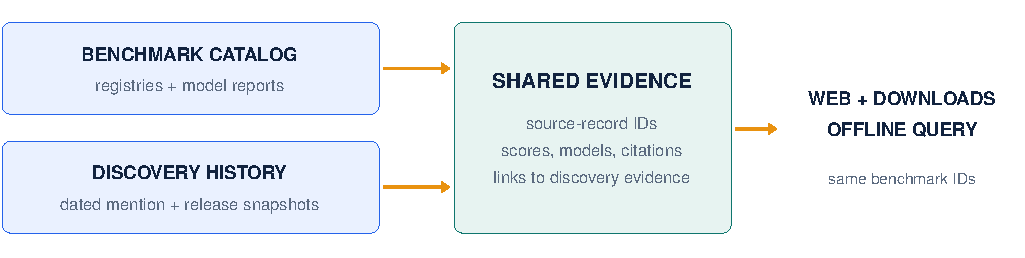
\includegraphics[width=\textwidth]{pipeline-evaluation.pdf}
\captionof{figure}{Two input paths support publication: dated discovery snapshots preserve mention and release evidence, while benchmark registries and model reports populate the shared catalog. Clients use the catalog's stable source-record IDs.}
\label{fig:pipeline}
\end{minipage}
\end{center}

Table~\ref{tab:reader-questions} describes the interfaces. Search and exports retain the full catalog; display filters affect only the selected view.

\begin{center}
\begin{minipage}{\textwidth}
\centering\small
\begin{tabularx}{\textwidth}{L{0.18\textwidth}Y Y}
\toprule
\textbf{Interface} & \textbf{Reader question} & \textbf{Evidence and scope}\\
\midrule
\href{https://benchmark-radar.org/}{Today} & What appeared or changed? & Daily discovery observations, source health, and links.\\
\href{https://benchmark-radar.org/saturation}{Search} & Which benchmarks match this task? & The complete catalog, including unscored records.\\
\href{https://benchmark-radar.org/leaderboard/}{Leaderboard} & Which evaluations combine lower scores with broader measured use? & Scored source records; distinct scored models or cited documents supply the selected count.\\
\href{https://benchmark-radar.org/saturation}{Saturation} & What scores and settings were reported? & Benchmark browsing and complete score histories; search reaches every source and year.\\
\href{https://benchmark-radar.org/blog}{Blog} & Can I read and share a daily brief? & Daily briefs and an archive built from committed discovery snapshots.\\
\href{https://benchmark-radar.org/cli}{CLI} & Can I inspect the same evidence locally? & The offline query client uses the same benchmark IDs and stable JSON response format.\\
\bottomrule
\end{tabularx}
\captionof{table}{Reader questions and evidence scope.}
\label{tab:reader-questions}
\end{minipage}
\end{center}



\subsection{Preserve Records Before Comparing Measurements}

A source record is one benchmark entry from one contributing source. We normalize names, identifiers, artifact links, score observations, model identities, and cited documents into common fields. A record remains in the catalog if a score, date, or citation is absent. Reviewed identity links connect related records while preserving their separate observations and counts.

Daily discovery contributes a different kind of evidence: collected mentions, releases, and updates. Exact identifiers such as DOIs, arXiv IDs, and repository URLs link those observations to artifacts. Discovery observations do not increase the benchmark catalog total. Appendix~\ref{app:operations} records detailed collection settings and display filters; Appendix~\ref{app:source-inventory} records source health at the cutoff.

\subsection{Retrieve Candidates with Their Evidence}

The same benchmark IDs reach web search, detail pages, dataset exports, and offline clients. Lexical search uses BM25F, a field-weighted word-matching score \citep{robertson2004bm25f}, with bounded boosts for name and phrase matches. Each result exposes matched and missing query words, the fields they occur in, and the score components. Source membership does not change the ranking. A shared query service supplies the CLI and HTTP interfaces with the same response format and local data provenance.

Candidate retrieval precedes suitability judgment. An analyst or agent can try focused query variants, inspect a record's tasks and score settings, and follow its citations. The interface preserves the evidence needed for that review. This paper evaluates catalog and measurement coverage; the contributor case illustrates usage without measuring retrieval accuracy or time saved.

\subsection{Audit the Full Population}
\label{sec:census-method}

The census starts with every record in the rebuilt catalog index and reads its detail file. It applies no date, score, or interface filter. We count finite numeric score observations once by observation ID. Within each benchmark record, we count scored models by source model ID, preserving separately evaluated configurations, and cited documents by document ID. Repeated observations do not create additional models or documents. The global model registry uses its recorded identity links; per-benchmark model counts are not summed into a global total.

Eligibility depends on the measurement a calculation needs. A declared percentage unit, known score direction, and numeric values within 0--100 permit a percentage-scale summary. Rescaling a displayed value or reading an aggregator's declared maximum does not establish that unit. Matching scales also do not establish matching test versions, prompts, tools, attempts, or evaluators.

Date coverage counts valid recorded benchmark release dates. Score entries retain their own date basis, including model announcements and document publication. We do not substitute those dates for an evaluation date. Appendix~\ref{app:reproducibility} provides the software revision, input hashes, census script, and validation procedure.

\section{Results}
\label{sec:results}

Appendix~\ref{app:full-catalog} provides the complete linked census; Appendix~\ref{app:measurement-coverage} details document, model, score, and date coverage.

\subsection{Catalog Coverage and Task Materials}

The rebuilt catalog contains \ReportNumber{\ReportCatalogCount} source records across \ReportCatalogSourceCount{} sources. We found \ReportNumber{\CensusNumericScores} numeric score observations on \CensusScored{} records, with \CensusUnscored{} records lacking numeric scores (Table~\ref{tab:catalog-coverage}). Two sources can describe a related benchmark, and we retain both source records.

\begin{center}
\begin{minipage}{\textwidth}
\centering\small
\begin{tabular}{lrrrr}
\toprule
\textbf{Source} & \textbf{Records} & \textbf{Scored} & \textbf{Unscored} & \textbf{Numeric scores}\\
\midrule
\CensusSourceRows
\midrule
\textbf{Total} & \textbf{\ReportNumber{\CensusRecords}} & \textbf{\CensusScored} & \textbf{\CensusUnscored} & \textbf{\ReportNumber{\CensusNumericScores}}\\
\bottomrule
\end{tabular}
\captionof{table}{Score coverage across the full catalog: \CensusScored{} records have numeric observations and \CensusUnscored{} do not. Scores count observations, not distinct models.}
\label{tab:catalog-coverage}
\end{minipage}
\end{center}

Of the \CensusUnscored{} unscored records, \CensusNoScoreWithLinks{} have at least one paper, repository, or dataset link. In the full catalog, \CensusPaperLinks{} records link to papers, \CensusRepoLinks{} to repositories, and \CensusDatasetLinks{} to datasets. A record can contain more than one type of link. For example, the OpenCompass Hub record for A-Bench links a paper, code repository, and dataset despite having no archived score.

For scored records, Figure~\ref{fig:leaderboard-frontier} lets readers browse by date, reported score, and number of scored models. Figure~\ref{fig:hle-scores} shows the reported model scores within one source record.

\begin{center}
\begin{minipage}{\textwidth}
\centering
\href{https://benchmark-radar.org/leaderboard/}{\includegraphics[width=0.85\textwidth]{leaderboard-frontier.png}}
\captionof{figure}{Benchmark Frontier on the Leaderboard page. The view combines reported scores, scored-model counts, and benchmark release dates or first-score date proxies. Gold rings mark the interface's Pareto candidates; hollow marks flag unverified scales or counts, and dotted outlines flag model-release date proxies. Click the image to explore the view.}
\label{fig:leaderboard-frontier}
\end{minipage}
\end{center}

\begin{center}
\begin{minipage}{\textwidth}
\centering
\href{https://benchmark-radar.org/saturation/?lscore=70&lfrontier=artificial-analysis-humanitys-last-exam}{\includegraphics[width=0.70\textwidth]{hle-score-history.png}}
\captionof{figure}{Inspecting Humanity's Last Exam in Benchmark RADAR. This Artificial Analysis record contains \FindingsHleAAScores{} reported scores; the highest displayed score is \FindingsHleDisplayMax{}. Marks identify model organizations, and the line connects successive best scores ordered by model release date. Click the image to open the interactive view.}
\label{fig:hle-scores}
\end{minipage}
\end{center}

\subsection{Benchmark Taxonomy Across the Full Catalog}
\label{sec:taxonomy}

Every source record also carries a capability label. We classify all \ReportNumber{\CensusRecords} records into \TaxonomyLevelOneCount{} top-level domains and \TaxonomyLevelTwoCount{} sub-domains (Figure~\ref{fig:taxonomy-sankey}). Labels come from the publishers' own fields---OpenCompass Hub dimensions, LLM Stats categories, Artificial Analysis categories, and the model-report registry domains---so \ReportNumber{\TaxonomyLabelledFromTags} records carry a label that traces to a named source field. The remaining \TaxonomyUnclassified{} records are LLM Stats community rows whose crawl supplied no description, category, or modality; we record that reason rather than assigning a class from the title.

Interaction paradigm and input modality are recorded as \emph{facets}: properties held beside a record's domain rather than inside it, so every record carries exactly one Level~1 class and, independently, any number of facet values. Facets therefore overlap each other and the Level~1 classes, and their counts do not sum to the population.

The separation matters because a benchmark that resolves repository issues is a coding benchmark run as an agent, not an agent benchmark. Of the \TaxonomyAgentic{} agentic records, \TaxonomyAgenticPrimary{} take Agentic \& Tool Use as their Level~1 class and \TaxonomyAgenticCoding{} sit under Coding \& Software Engineering, with the rest spread across \TaxonomyAgenticOtherClasses{} further classes. A scheme with one axis has to choose, and choosing the domain hides those \TaxonomyAgenticCoding{} records from any count of agentic evaluation.

\begin{center}
\begin{minipage}{\textwidth}
\centering
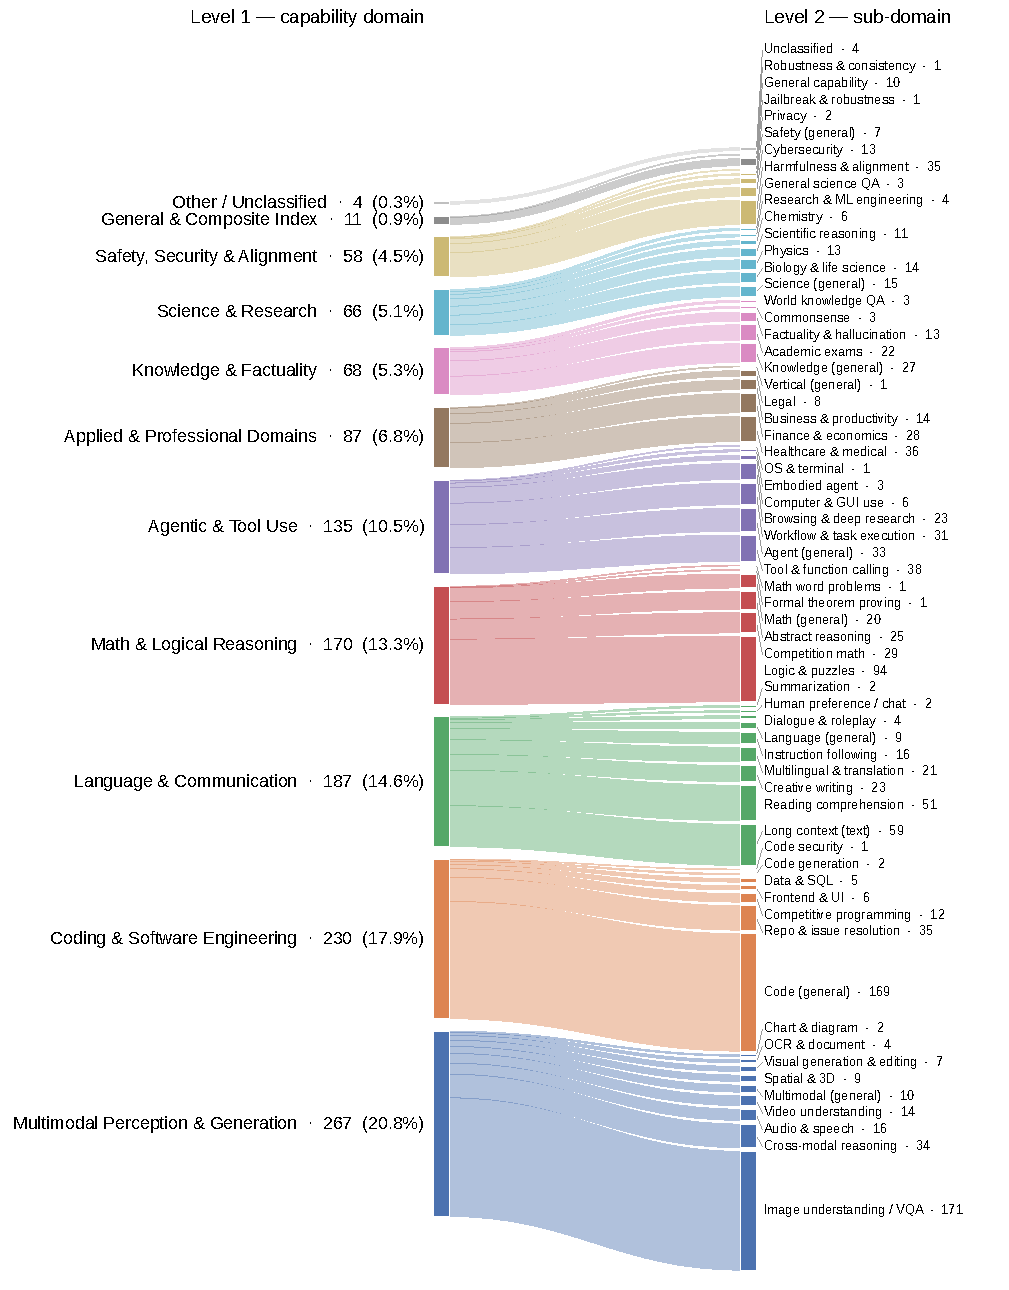
\includegraphics[width=\textwidth]{taxonomy-sankey.pdf}
\captionof{figure}{Capability taxonomy over the full catalog. Ribbon height is one unit per source record, so both columns carry all \ReportNumber{\CensusRecords} records. Level~1 is one primary label per record; interaction paradigm and modality are recorded as separate facets and are not drawn here.}
\label{fig:taxonomy-sankey}
\end{minipage}
\end{center}

Figure~\ref{fig:taxonomy-trends} places the \CensusReleaseKnown{} records that carry a benchmark release date on their release year. The \FindingsMissingRelease{} records without one keep their classification in a separate column rather than leaving the figure. A year's share is read only where the evidence supports one, which takes more than a sufficient count: the OpenCompass Hub crawl stops at the discovery cutoff, so the truncated final year is drawn mostly from model reports and its share would measure the change of catalog rather than a change in the field. We therefore also require a year's source mix to stay close to the pooled mix. Over the reported years that mix is stable, and reweighting each year to a common source composition moves the agentic share by at most \TaxonomyMixAdjustment{} percentage points, so the rise is not an artifact of which catalog supplied a given year's records.

\begin{center}
\begin{minipage}{\textwidth}
\centering
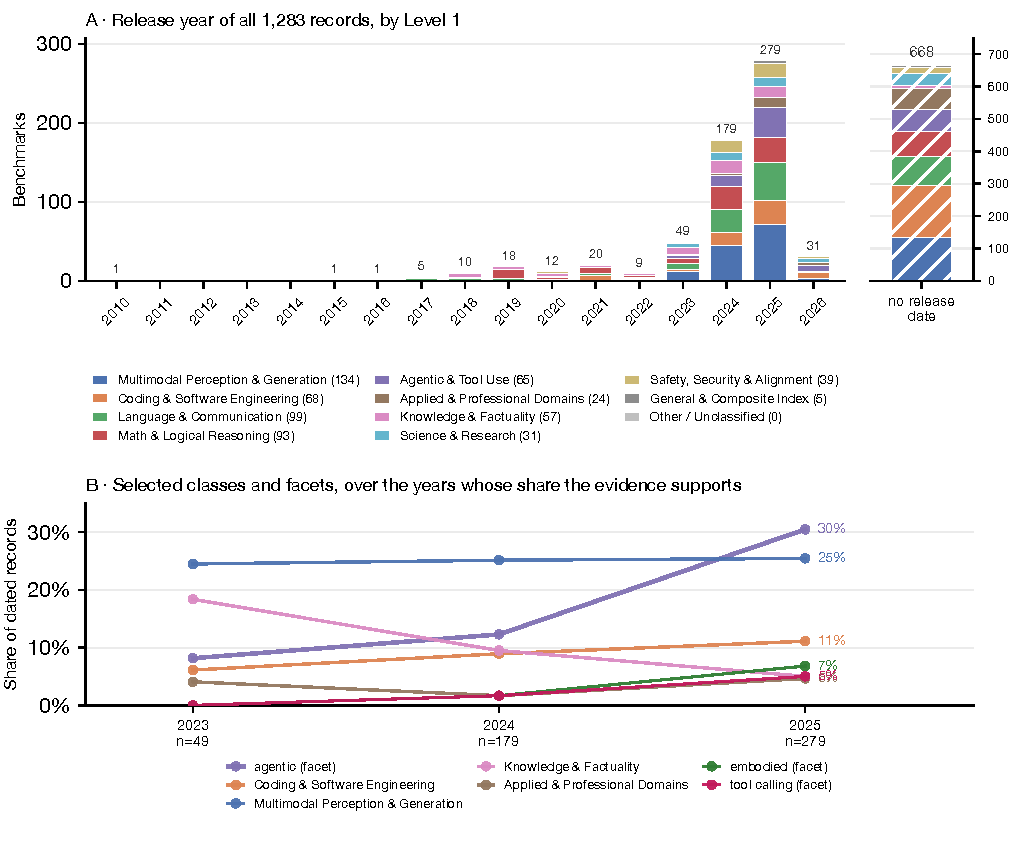
\includegraphics[width=\textwidth]{taxonomy-trends.pdf}
\captionof{figure}{Release-year composition of the classified catalog. Panel~A holds every record: \CensusReleaseKnown{} on the year axis and \FindingsMissingRelease{} in the undated column, which carries its own scale. Panel~B reports shares only for years with at least \TaxonomyMinYearRecords{} dated records and a source mix close to the pooled one; the excluded years hold \TaxonomyExcludedFromShares{} dated records between them and remain counted in Panel~A. Series marked \emph{facet} are cross-cutting properties rather than Level~1 classes, so the lines in Panel~B overlap and do not sum to 100\%.}
\label{fig:taxonomy-trends}
\end{minipage}
\end{center}

\subsection{Discovery Coverage Alongside the Catalog}

The daily discovery collection contains \ReportNumber{\ReportObservationCount} observations and \ReportNumber{\ReportArtifactCount} artifacts linked by exact identifiers across \ReportSnapshotCount{} snapshots. \CensusSimulatedSnapshots{} snapshots are simulated historical backfills; their dates describe reconstructed collection windows. These discovery units remain separate from benchmark records.

Five discovery source labels account for \ReportNumber{\FindingsTopFiveObservations} of \ReportNumber{\ReportObservationCount} observations (\FindingsTopFiveShare\%). Figure~\ref{fig:source-composition} includes the remaining labels in one aggregate bar. Source caps and collection failures can affect this mix. Of the \ReportNumber{\ReportArtifactCount} artifacts, \CensusMultisourceArtifacts{} have observations from multiple sources. Missing or inconsistent identifiers may prevent additional cross-source matches.

\begin{center}
\begin{minipage}{\textwidth}
\centering
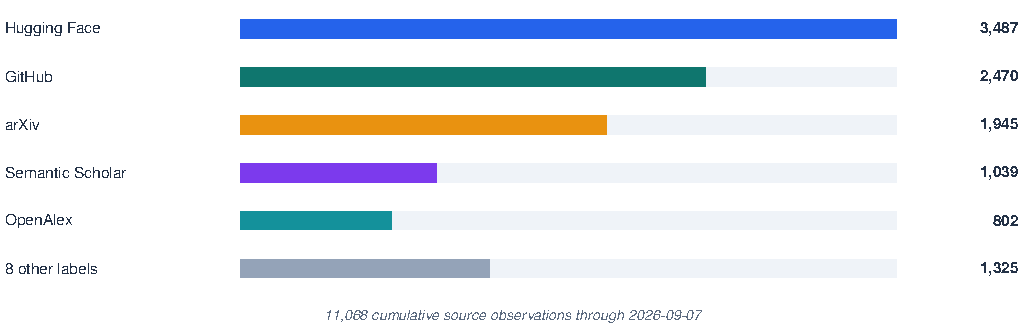
\includegraphics[width=0.92\textwidth]{source-composition.pdf}
\captionof{figure}{Discovery observations by source through \datacutoff{}. Repeat sightings count as observations.}
\label{fig:source-composition}
\end{minipage}
\end{center}


Figure~\ref{fig:discovery-trends} complements source coverage with the daily reading view. Its category cards separate new releases from updates, while the chart exposes changes in surfaced evidence and attention alongside collection failures.

\begin{center}
\begin{minipage}{\textwidth}
\centering
\href{https://benchmark-radar.org/trends/}{\includegraphics[width=\textwidth]{discovery-trends.png}}
\captionof{figure}{Discovery trends through September 7, 2026. Category cards show newly surfaced releases and track updates separately; the bars show daily evidence and attention volume. Category tags overlap. The visible coverage notice reports failed sources. Click the image to open Trends.}
\label{fig:discovery-trends}
\end{minipage}
\end{center}

\clearpage
\section{Worked Example: Checking Prior Art}
\label{sec:worked-example}

Before designing a new evaluation, a contributor surveyed August work on credit assignment in agentic training, with small Qwen-series models as a requirement for reproducible baselines. A coding agent installed the Benchmark RADAR client and its public Skill, downloaded the corpus, and searched locally. It inspected the recorded paper, repository, and dataset links, tried additional web searches for work described in different terms, and read the source evidence before assembling the related-work table in Table~\ref{tab:use-case-survey}.

The contributor used the table to assess whether the proposed evaluation duplicated existing work. The workflow separates candidate retrieval from comparison: Benchmark RADAR retrieves candidates and exposes their evidence; the researcher or agent judges their relevance and compares the designs. Appendix~\ref{app:use-case} retains the session screenshots and an earlier manually assembled comparison.

\begin{center}
\begin{minipage}{\textwidth}
\centering
\footnotesize
\setlength{\tabcolsep}{3pt}
\renewcommand{\arraystretch}{1.25}
\resizebox{0.98\textwidth}{!}{%
\begin{tabular}{L{0.45cm}L{3.05cm}L{1.65cm}L{2.35cm}L{3.45cm}L{2.55cm}L{2.9cm}}
\toprule
\textbf{\#} & \textbf{Work} & \textbf{Published} & \textbf{Qwen base model(s)} & \textbf{Credit-assignment focus} & \textbf{Agentic benchmarks used} & \textbf{Link} \\
\midrule
1 & SRPO: Self-Reflective Policy Optimization for Long-Horizon Reasoning & 2026-08-25 & Qwen3-8B (also Qwen3-1.7B / 32B scaling) & Reflection-conditioned dense token-level signals convert sparse terminal reward into training signal & AIME'24, WebShop, ALFWorld, SWE-Bench-Lite & \url{https://arxiv.org/abs/2608.23493} \url{https://github.com/Galleons2029/SRPO} \\
2 & ContextPilot: Teaching Agents for Proactive Context Management via Fine-grained RL & 2026-08-28 & Qwen3-8B, Qwen3-14B & Coarse-grained $\rightarrow$ action-level credit assignment over branched trajectories during agentic RL & InfBench (InfiniteBench), NovelQA, LongMemEval, BrowseComp+ & \url{https://arxiv.org/abs/2608.28476} \url{https://github.com/Tencent/ContextPilot} \\
3 & SkillGate: Training In-Policy Skill Selection in Long-Horizon Agents & 2026-08-21 & Qwen3.5-9B (SFT checkpoint, RL init) & Selector credit starvation; partitions token support into two credit channels (outcome vs.\ action-local advantage) & 5 agentic benchmarks incl.\ SkillsBench, SWE (16-candidate skill slate) & \url{https://arxiv.org/abs/2608.18852} \\
4 & CIPO: Contextual Information Policy Optimization for Search Agents & 2026-08-06 & Qwen2.5-3B-Instruct, Qwen2.5-7B-Instruct & Dense turn-level credit (EALR) to evidence-using reasoning actions, combined with outcome reward & HotpotQA, 2WikiMultiHopQA, MuSiQue, Bamboogle + 3 OOD & \url{https://arxiv.org/abs/2608.06128} \\
5 & MoRSE: Task-Oriented Multi-Agent System with Mixture of Role-Subtask Experts & 2026-08-10 & Qwen3-4B-Instruct (one of three backbones; also Llama-3.1-8B, Gemma-4-31B) & Hierarchical GRPO with two-layer credit assignment (isolates expert vs.\ routing quality) & Code-generation benchmarks (multi-agent), held-out task domains & \url{https://arxiv.org/abs/2608.09251} \\
\bottomrule
\end{tabular}%
}
\captionof{table}{Summary table of recent work on credit assignment in agentic training, assembled during the session. Each row links to its arXiv record and, where available, its repository.}
\label{tab:use-case-survey}
\end{minipage}
\end{center}



\section{Limitations and Future Work}
\label{sec:caveat-future-work}

The census describes this catalog at its recorded cutoff. Collection limits, failed requests, missing identifiers, and different snapshot dates affect its coverage. Source records are not a count of distinct underlying tests. Broader coverage requires additional source collection and review of the evidence already present.

Retrieval precision, task suitability, and time saved remain to be evaluated. The worked example combines local queries with web search and has no controlled baseline. Lexical matching can miss paraphrases and renamed tasks. Evaluating semantic retrieval \citep{reimers2019sentencebert} will require reviewed relevance judgments across queries and candidate records, including less familiar benchmark families.

The arXiv discovery route collects new submissions; it does not backfill papers first posted before the collection window when later versions appear. The searches used for Section~\ref{sec:related-work} missed two relevant earlier studies \citep{yang2026benchmark,akhtar2026plateau}, which a coauthor identified and read.

Measuring benchmark saturation or score stagnation requires comparable test versions and settings, with dates tied to score reporting or evaluation.

Task-capability classification also remains unvalidated in this rebuild. The deterministic null extractor used in CI assigns no capability levels to its \ReportNumber{\CensusUnclassified} discovery-derived tracks. Completing and evaluating those labels is a separate task from maintaining the benchmark catalog.

\section{Conclusion}

Benchmark RADAR brings daily benchmark discovery, catalog search, model-report mentions, and score histories into one living search engine. Readers can find candidate evaluations, locate task materials, inspect reporting choices, and follow the settings and citations behind a score. Shared benchmark IDs connect the web dashboard, downloadable catalog, and offline query clients.

The v0.11.0 release makes \ReportNumber{\CensusRecords} source records searchable and preserves \CensusNoScoreWithLinks{} unscored records with artifact links. Its full-catalog analyses distinguish benchmark records, scored models, cited documents, and numeric observations.

\section*{Author Contributions}
\label{sec:author-contributions}

Koutian Wu led the work and manuscript preparation, built the initial collection pipeline, and implemented data aggregation across sources. Junjie Zhou prepared the score-archive audit and contributed report revisions. Ergan Shang prepared figures and contributed copyediting. Jiayu Wang contributed the worked use case and its supporting evidence. Pengqian Han contributed data analysis and copyediting. Wanghan Xu contributed review and copyediting. Junkai Wang contributed review and copyediting.

\begingroup
\small
\raggedright
\bibliographystyle{plainnat}
\bibliography{references}
\endgroup

\clearpage
\appendix
\begin{center}
{\LARGE\bfseries Appendix}
\end{center}
\vspace{0.75em}

\section{Full-Catalog Census}
\label{app:full-catalog}

This census retains all \ReportNumber{\CensusRecords} source records, including those without scores.

\begin{center}
\resizebox{0.98\textwidth}{!}{\input{figures/corpus-evidence-body.tex}}
\captionof{figure}{\CensusNoScoreWithLinks{} unscored entries provide artifact links. Each mark represents one source record and links to its detail page. All \ReportNumber{\CensusRecords} records appear, without a date or score filter.}
\label{fig:corpus-evidence}
\end{center}

\section{Catalog Evidence and Measurement Coverage}
\label{app:measurement-coverage}

The following analyses use the same catalog as Section~\ref{sec:results}. They document the evidence behind its records and the requirements for comparing measurements.

\subsection{Cited Documents and Scored Models}

The common document registry contains \ReportNumber{\CensusDocuments} distinct cited documents, attached to \ReportNumber{\CensusDocumentsKnown} of the \ReportNumber{\CensusRecords} benchmark records. \FindingsMissingDocuments{} records have no cited documents. The shared model registry contains \CensusModels{} model identities. Model identifiers are available for every numeric score in all \CensusScored{} scored records, allowing distinct models to be counted within each record. For unscored records, this count is unknown.

Table~\ref{tab:model-document-coverage} illustrates why these counts cannot substitute for one another. The Artificial Analysis record for GPQA Diamond contains scores for \FindingsGpqaAAModels{} models and cites \FindingsGpqaAADocuments{} registry page. The Model reports record cites \FindingsGpqaReportsDocuments{} documents and contains \FindingsGpqaReportsScores{} numeric observations for \FindingsGpqaReportsModels{} models.

\begin{center}
\begin{minipage}{\textwidth}
\centering\small
\begin{tabularx}{\textwidth}{Y L{0.25\textwidth}rrr}
\toprule
\textbf{Benchmark record} & \textbf{Source} & \textbf{Models} & \textbf{Documents} & \textbf{Scores}\\
\midrule
\FindingsModelDocumentRows
\bottomrule
\end{tabularx}
\captionof{table}{One cited page can document hundreds of scored models. Models count distinct source model IDs within a record; documents count distinct citation IDs; scores count numeric observations. These selected examples illustrate the units. The census retains all source records.}
\label{tab:model-document-coverage}
\end{minipage}
\end{center}

Table~\ref{tab:model-document-coverage} also records \FindingsHleAAModels{} scored models for Humanity's Last Exam, \FindingsSciCodeAAModels{} for SciCode, and \FindingsCritPtAAModels{} for CritPt, each under one Artificial Analysis citation.

\subsection{Score Scales and Comparison Eligibility}

Only \CensusPercent{} of the \CensusScored{} scored records declare a percentage unit with a known direction and values within 0--100. The remaining \CensusOtherNumeric{} scored records use other or unverified scales. We retain their numeric observations, which do not support a shared percentage-headroom calculation. Table~\ref{tab:measurement-coverage} accounts for the entire catalog before any such comparison.

\begin{center}
\begin{minipage}{\textwidth}
\centering\small
\begin{tabularx}{\textwidth}{Y r L{0.46\textwidth}}
\toprule
\textbf{Measurement state} & \textbf{Records} & \textbf{Interpretation}\\
\midrule
Numeric scores, declared percentage scale & \CensusPercent & Supports scale-specific summaries; protocols still need checking.\\
Numeric scores, other or unverified scale & \CensusOtherNumeric & Retain scores; do not assume a 100-point ceiling.\\
No numeric score & \CensusUnscored & Score headroom remains unknown.\\
\midrule
Full population & \ReportNumber{\CensusRecords} & Every source record remains in the census.\\
\bottomrule
\end{tabularx}
\captionof{table}{Only \CensusPercent{} of \CensusScored{} scored records meet the percentage-scale rule in Section~\ref{sec:census-method}. All \ReportNumber{\CensusRecords} records remain accounted for.}
\label{tab:measurement-coverage}
\end{minipage}
\end{center}

The catalog records benchmark release dates for \CensusReleaseKnown{} records, leaving \FindingsMissingRelease{} without a release date. Across score observations, \ReportNumber{\FindingsModelDateScores} entries carry model-announcement dates and \FindingsDocumentDateScores{} carry document-publication dates. Neither date basis directly establishes an evaluation date. Researchers must first establish dates and comparable evaluation settings for the relevant source records.

A small gap to a metric ceiling can describe a reported setup. Catalog-wide headroom or recency estimates require the eligible measurement coverage alongside the statistic.

\newpage
\subsection{Documentation Across All Catalog Sources}

The documentation analysis covers all \ReportNumber{\FindingsRecords} benchmark records. It finds \ReportNumber{\CensusDocuments} distinct cited documents supporting \ReportNumber{\CensusDocumentsKnown} records; \FindingsMissingDocuments{} records have no cited document. Table~\ref{tab:report-mentions} includes every source and keeps benchmark records separate from document counts. A registry page and a model report both count as one cited document when attached to a record. Repeated citations to the same document do not increase its count.

\begin{center}
\begin{minipage}{\textwidth}
\centering\small
\begin{tabularx}{\textwidth}{Y r r r r}
\toprule
\textbf{Source} & \textbf{Records} & \textbf{With docs} & \textbf{Documents} & \shortstack[r]{\textbf{Docs without}\\\textbf{named org.}}\\
\midrule
\FindingsDocumentRows
\midrule
Total & \ReportNumber{\CensusRecords} & \ReportNumber{\CensusDocumentsKnown} & \ReportNumber{\CensusDocuments} & \ReportNumber{\FindingsDocumentsUnknownOrganization}\\
\bottomrule
\end{tabularx}
\captionof{table}{Documentation across the complete v0.11.0 catalog. ``With docs'' counts benchmark records; the last two columns count distinct documents. Missing organization metadata remains unknown.}
\label{tab:report-mentions}
\end{minipage}
\end{center}

Documentation is widespread, but the release data does not identify an organization for \ReportNumber{\FindingsDocumentsUnknownOrganization} cited documents. The complete export retains each document's identity and source URL on its benchmark record.

\subsection{Reported Scores Across the Full Catalog}
\label{sec:headroom}

The score analysis retains all \ReportNumber{\FindingsRecords} records and their \ReportNumber{\CensusNumericScores} numeric observations. Table~\ref{tab:reported-headroom} summarizes scored-model coverage for each source. \FindingsBroadModelRecords{} benchmark records contain numeric scores for at least 100 distinct source model IDs. The \CensusOtherNumeric{} records on other or unverified scales contribute their scores and model counts on the same terms as percentage-scale records. The \CensusUnscored{} records without numeric scores remain in the population with unknown scored-model coverage.

\begin{center}
\begin{minipage}{\textwidth}
\centering\small
\begin{tabularx}{\textwidth}{Y r r r r r r}
\toprule
\textbf{Source} & \textbf{Records} & \textbf{Scored} & \textbf{Unscored} & \shortstack[r]{\textbf{Score}\\\textbf{rows}} & \shortstack[r]{\textbf{Median}\\\textbf{models}} & \shortstack[r]{\textbf{Max.}\\\textbf{models}}\\
\midrule
\FindingsScoreRows
\midrule
Total & \ReportNumber{\CensusRecords} & \CensusScored{} & \CensusUnscored{} & \ReportNumber{\CensusNumericScores} & & \\
\bottomrule
\end{tabularx}
\captionof{table}{Reported scores across every source in the v0.11.0 release. Models count distinct source model IDs within each benchmark record. Medians and maxima use records with known model counts; unscored records are not assigned zero models. Model counts are not summed across benchmarks. The record-level score export contains every catalog record, including raw maxima, all tied reporting models and citations, units, settings, and explicit missing values.}
\label{tab:reported-headroom}
\end{minipage}
\end{center}

The accompanying \texttt{evidence/catalog-findings.csv} contains one row per benchmark record, with a JSON counterpart retaining detailed evidence. Each scored record has its highest numeric value on the source's native scale and every tied score observation. Units and score direction remain attached to that record; a numeric maximum need not be the best result for a lower-is-better metric. Display multipliers are recorded separately and do not establish a percentage unit.

Percentage headroom remains a separate calculation: 100 minus a record's highest value, only when its unit is explicitly percent, its direction is higher-is-better, and its values stay within 0--100. Missing scale evidence leaves headroom unknown while preserving the scores themselves. The export records eligibility for every benchmark. Test versions, reasoning budgets, tools, attempts, and evaluators must still be checked before comparing results \citep{gebru2021datasheets,mitchell2019modelcards}.

\subsection{Date Evidence Across the Full Catalog}

The date analysis also retains all \ReportNumber{\FindingsRecords} source records. Table~\ref{tab:score-coverage-gaps} separates benchmark release dates from dates attached to numeric observations. A known model announcement date supplies a source-record proxy, not an evaluation date.

\begin{center}
\begin{minipage}{\textwidth}
\centering\small
\begin{tabularx}{\textwidth}{Y r r r r r}
\toprule
\textbf{Source} & \textbf{Records} & \shortstack[r]{\textbf{Release}\\\textbf{known}} & \shortstack[r]{\textbf{Doc.-dated}\\\textbf{scores}} & \shortstack[r]{\textbf{Model-dated}\\\textbf{scores}} & \shortstack[r]{\textbf{Undated}\\\textbf{scores}}\\
\midrule
\FindingsDateRows
\midrule
Total & \ReportNumber{\CensusRecords} & \CensusReleaseKnown{} & \FindingsDocumentDateScores{} & \ReportNumber{\FindingsModelDateScores} & \FindingsUndatedScores{}\\
\bottomrule
\end{tabularx}
\captionof{table}{Date evidence for the complete v0.11.0 catalog. The first two numeric columns count benchmark records; the final three count numeric score observations. Records with no scores remain in the Records column.}
\label{tab:score-coverage-gaps}
\end{minipage}
\end{center}

The exported rows preserve each record's release date and the date basis of its scores. A study of score progress needs actual reporting or evaluation dates and comparable settings for the records being studied.

\section{Collection Settings and Display Filters}
\label{app:operations}

The \datacutoff{} snapshot records \ReportNumber{\FindingsRunFetched} fetched rows and \FindingsRunDeduplicated{} candidates after duplicate removal. Of these, \FindingsRunPublished{} qualified for publication and \FindingsRunRecommended{} met the recommendation threshold. These are discovery-run counts, separate from the benchmark catalog census. Published evidence retains source URLs, retrieval times, parser versions, identifiers, and payload checksums. Raw responses and credentials remain outside the public artifact.

Benchmark Frontier, on the Leaderboard tab, requires a numeric score and excludes known pre-2024 benchmarks. It retains scored records with unknown dates or counts through labelled marks, and keeps unverified scales outside Pareto calculations. Its initial score cutoff is 70. The linked score ranking retains its date and numeric-score requirements independently of that cutoff. General catalog search and exports retain the full population. The census in this paper applies none of these display filters.

A separate priority score for daily recommendations combines relevance (35\%), evidence (20\%), recency (20\%), and adoption (25\%) on a 0--100 scale. These weights describe reading priority for discovery observations. An agent assessing benchmark suitability can try focused query variants, inspect record details, and read the cited sources; that judgment occurs after candidate retrieval.

\section{Source Inventory and Health}
\label{app:source-inventory}

Table~\ref{tab:healthy-connectors} lists source connectors that completed successfully at the cutoff. Row counts are measured before duplicate removal and ranking. A connector can be healthy with zero eligible rows if its request succeeds and the response can be parsed. Core sources cover papers, shared model or dataset artifacts, and code; all must be healthy before publication. Failures in optional sources are reported but do not block publication.

\begin{center}
\begin{minipage}{\textwidth}
\centering
\small
\begin{tabularx}{\textwidth}{L{0.21\textwidth}Y L{0.21\textwidth}L{0.08\textwidth}}
\toprule
\textbf{Connector} & \textbf{Role} & \textbf{Cutoff status} & \textbf{Core}\\
\midrule
arXiv & Primary papers via selected AI, language, vision, and software categories & Healthy; \FindingsConnectorArxiv{} rows & Yes\\
Hugging Face Hub & Datasets and Spaces connected to benchmark artifacts & Healthy; \FindingsConnectorHuggingface{} rows & Yes\\
GitHub Search & Code repositories and benchmark artifacts & Healthy; \FindingsConnectorGithub{} rows; at cap & Yes\\
GitHub Organizations & Reviewed organization repositories & Healthy; \FindingsConnectorGithubOrganizations{} rows & No\\
Hugging Face Papers & Community-surfaced papers & Healthy; \FindingsConnectorHuggingfacePapers{} rows & No\\
Kaggle Datasets & Public benchmark datasets & Healthy; \FindingsConnectorKaggleDatasets{} rows & No\\
Zenodo & DOI-bearing research artifacts & Healthy; \FindingsConnectorZenodo{} rows & No\\
Crossref & DOI metadata & Healthy; \FindingsConnectorCrossref{} rows & No\\
OpenReview & Conference submissions & Healthy; no eligible rows & No\\
GitHub Releases & First-party releases & Healthy; \FindingsConnectorGithubReleases{} row & No\\
OpenAlex & Scholarly discovery metadata & Healthy; \FindingsConnectorOpenalex{} rows & No\\
\bottomrule
\end{tabularx}
\captionof{table}{Healthy direct discovery connectors at the current cutoff.}
\label{tab:healthy-connectors}
\end{minipage}
\end{center}

Table~\ref{tab:first-party-feeds} lists research and engineering feeds operated by the institutions being monitored. They can surface benchmark papers, datasets, model announcements, and engineering posts. The feed collector returned no records at the cutoff. Semantic Scholar returned a malformed payload, and Brave Search lacked an API key. These optional-route failures remain recorded in the snapshot. Searches restricted to an organization's website cover institutions that lack a verified feed.

\begin{center}
\begin{minipage}{\textwidth}
\centering
\small
\begin{tabularx}{\textwidth}{Y Y}
\toprule
\textbf{Feeds 1-12} & \textbf{Feeds 13-24}\\
\midrule
Meituan Engineering & Ai2\\
OpenAI News & Together AI\\
Google AI & Sakana AI\\
Google DeepMind & Qwen\\
Google Research & Ollama\\
Apple Machine Learning Research & Stability AI\\
AWS Machine Learning & Nomic AI\\
Hugging Face Blog & Replicate\\
Microsoft Research & NVIDIA Developer\\
NVIDIA AI Blog & IBM Research\\
Mistral AI & Databricks\\
Meta Research & LangChain\\
\bottomrule
\end{tabularx}
\captionof{table}{First-party research and engineering feeds monitored by Benchmark Radar.}
\label{tab:first-party-feeds}
\end{minipage}
\end{center}

\section{Worked Use Case: Prior-Art Check for a New Evaluation}
\label{app:use-case}

The contributor wanted to determine whether a proposed evaluation duplicated existing work. They surveyed work published in August 2026 on credit assignment in agentic training, using small Qwen-series models as a requirement for reproducible baseline experiments. The search produced a focused comparison table that the contributor used to assess the proposed design.

The contributor gave the task to a coding agent together with the public setup instructions for Benchmark Radar. The agent installed the command-line client and the Benchmark Radar Skill, a set of instructions for using the client. It then downloaded the local corpus and queried candidate records offline (Figure~\ref{fig:use-case-session}).

\begin{center}
\begin{minipage}{\textwidth}
\centering
\includegraphics[width=0.92\textwidth]{agent-session.png}
\captionof{figure}{A coding agent installs the Benchmark Radar client and its usage instructions, then runs local queries.}
\label{fig:use-case-session}
\end{minipage}
\end{center}

The agent inspected paper, repository, and dataset links to decide which sources to open next. Figures~\ref{fig:use-case-paper} and~\ref{fig:use-case-code} show two retrieved discovery records: one has a repository link, and the other has both paper and repository links. Neither records a dataset link, leaving dataset availability for a follow-up check.

\begin{center}
\begin{minipage}{\textwidth}
\centering
\includegraphics[width=0.92\textwidth]{artifact-status-paper.png}
\captionof{figure}{A retrieved discovery record with a repository link for inspecting the implementation. Paper and dataset links are missing from the record.}
\label{fig:use-case-paper}
\end{minipage}
\end{center}

\begin{center}
\begin{minipage}{\textwidth}
\centering
\includegraphics[width=0.92\textwidth]{artifact-status-code.png}
\captionof{figure}{A second discovery record provides both paper and repository links. Its dataset link needs a follow-up check.}
\label{fig:use-case-code}
\end{minipage}
\end{center}

The agent supplemented local queries with web search to find related work described in different terms. It cross-checked the candidate sets and inspected the source evidence before selecting records for the comparison. Figure~\ref{fig:use-case-cross} shows the word matches and score components available for inspecting one retrieved candidate.

\begin{center}
\begin{minipage}{\textwidth}
\centering
\includegraphics[width=0.92\textwidth]{cross-validation.png}
\captionof{figure}{A candidate record with query-word matches and retrieval-score components for the agent to inspect when judging relevance.}
\label{fig:use-case-cross}
\end{minipage}
\end{center}

The resulting related-work table appears in Table~\ref{tab:use-case-survey} in the main text.

Table~\ref{tab:benchmark-comparison} shows a prior-art comparison table from an earlier benchmark-design effort by one contributor. Each row is one related benchmark and each column one design dimension, with each cell read from a source paper. The contributor reported that assembling it took more effort than any part of that project except producing the benchmark data. Benchmark Radar retrieves candidates for this kind of comparison and exposes the matching words and fields for inspection; the comparison itself requires reading the source evidence.

\begin{center}
\begin{minipage}{\textwidth}
\centering
\setlength{\tabcolsep}{3pt}
\renewcommand{\arraystretch}{1.2}
\resizebox{0.98\textwidth}{!}{%
\begin{tabular}{l c c c c c c}
\toprule
\textbf{Bench Name} & \textbf{End-to-End Tasks} & \textbf{Fine-Grained Eval} & \textbf{Researcher-Quality Eval} & \textbf{Data Generation} & \textbf{Multi-Harness Eval} & \textbf{\#Tasks} \\
\midrule
MLE-Bench~\citep{chan2025mle} & \xmark & \cmark & \xmark & Transfer\&Compose & \cmark & 75 \\
MLGym-Bench~\citep{nathani2025mlgym} & \xmark & \cmark & \xmark & Automatic & \xmark & 13 \\
EXP-Bench~\citep{kon2025exp} & \cmark & \xmark & \xmark & Automatic & \cmark & 461 \\
ResearchCodeBench~\citep{hua2026researchcodebench} & \xmark & \cmark & \xmark & Transfer\&Compose & \xmark & 212 \\
MLR-Bench~\citep{chen2026mlr} & \cmark & \xmark & \xmark & Automatic & \cmark & 201 \\
PaperBench~\citep{starace2025paperbench} & \xmark & \cmark & \xmark & Transfer\&Compose & \xmark & 8316 \\
AstaBench~\citep{bragg2025astabench} & \cmark & \cmark & \xmark & Transfer\&Compose & \cmark & 2400+ \\
InnovatorBench~\citep{wu2025innovatorbench} & \cmark & \xmark & \xmark & Transfer\&Compose & \xmark & 20 \\
AIRS-Bench~\citep{lupidi2026airs} & \xmark & \cmark & \xmark & Automatic & \cmark & 20 \\
COMPOSITE-Stem~\citep{waters2026composite} & \cmark & \cmark & \xmark & Manual & \xmark & 70 \\
ScienceBoard~\citep{sun2025scienceboard} & \xmark & \cmark & \xmark & Manual & \xmark & 169 \\
\bottomrule
\end{tabular}%
}
\captionof{table}{A prior-art comparison table assembled manually for an earlier benchmark-design effort. Each row is one related benchmark and each column one design dimension, all read from the source papers by hand.}
\label{tab:benchmark-comparison}
\end{minipage}
\end{center}

\clearpage
\section{Reproducibility, Access, and Citation}
\label{app:reproducibility}

This revision uses the \href{https://github.com/ktwu01/benchmark-radar/releases/tag/v0.11.0}{Benchmark Radar v0.11.0 release}, software commit \gitcommit{}, with a discovery cutoff of \datacutoff{}. The release preserves the inputs already audited for this paper; later data is outside its scope. A fresh detached checkout passed the six required CI steps in order: linting, formatting checks, catalog normalization, classification, release construction, and tests. The dated registry inputs remain the August snapshots registered in \texttt{data/leaderboard\_snapshots.yml}; the September cutoff does not imply that those sources were recrawled on that day.

The data build normalizes the registry and model-report inputs into the shared catalog, then classifies discovery tracks and packages the catalog with checksums. Installed clients validate an update before activating it. The manuscript and its dated analysis files build independently of the software checkout. The project provides a DOI and Citation File Format record for citation \citep{smith2016,katz2021,cff}. Table~\ref{tab:access-artifacts} lists the access and citation resources.

\begin{center}
\begin{minipage}{\textwidth}
\centering
\small
\begin{tabularx}{\textwidth}{L{0.28\textwidth}Y}
\toprule
\textbf{Artifact} & \textbf{Canonical or permanent location}\\
\midrule
Archived paper (v0.9.0) & \url{https://doi.org/10.5281/zenodo.22167102}\\
Release data (v0.11.0) & \url{https://github.com/ktwu01/benchmark-radar/releases/tag/v0.11.0}\\
Source code & \url{https://github.com/ktwu01/benchmark-radar}\\
Dashboard & \url{https://benchmark-radar.org/}\\
Discovery observations (JSON) & \url{https://benchmark-radar.org/data/radar.json}\\
Benchmark catalog & \url{https://benchmark-radar.org/data/benchmark-index.json}\\
RSS & \url{https://benchmark-radar.org/feed.xml}\\
Citation metadata & \url{https://github.com/ktwu01/benchmark-radar/blob/main/CITATION.cff}\\
\bottomrule
\end{tabularx}
\captionof{table}{Access and citation artifacts for Benchmark Radar.}
\label{tab:access-artifacts}
\end{minipage}
\end{center}

The census reads \texttt{site/data/benchmark-index.json}, the detail shards under \texttt{site/data/benchmarks/}, and the shared document and model registries. Discovery counts come from the rebuilt \texttt{site/data/radar.json} and dated snapshots. Model reports and score YAML files are normalization inputs, not a separate population for the paper's findings.

The paper repository contains \texttt{scripts/audit\_catalog.py}, which validates IDs and counts, computes the census, and exports \texttt{catalog-data.tex} plus \texttt{evidence/catalog-audit.json}. The JSON includes every source-record key, measurement state, per-record model and document counts, citation IDs, and SHA-256 hashes of the inputs. The script checks score-observation uniqueness, record-to-shard identity, document-registry coverage, and reconciliation of scored and unscored records. Its \texttt{--check} mode compares a fresh calculation against the committed outputs. Figure~\ref{fig:corpus-evidence} draws one linked dot per census record in source-key order.

Reproduce from a clean checkout at software commit \gitcommit{} using the README's six-step CI sequence. The software exporter writes \texttt{figure-data.tex}; the paper's \texttt{audit\_catalog.py} and \texttt{audit\_findings.py} take the rebuilt software path. The findings audit writes \texttt{findings-data.tex} and \texttt{evidence/catalog-findings.json} plus a CSV export. Every analysis retains exactly the catalog's source-record IDs. It records native score maxima and all tied observations, units, settings, cited documents, model counts, and date evidence. Table cells and repeated numeric claims are generated from these same inputs. Run each exporter's \texttt{--check} mode, build with \texttt{make arxiv}, compile the extracted package, and inspect the PDF. Normal builds use the committed inputs. The v0.9.0 DOI remains an earlier deposit; live dashboard counts require a retrieval date.

% \section{Licensing}
% Software: MIT License. The paper and original editorial content: CC BY-NC 4.0.
% Commercial republication, resale, paid newsletters, dataset packaging, or commercial
% product integration requires prior written permission from Koutian Wu. Third-party
% source material remains under its original terms.

\end{document}
